% Options for packages loaded elsewhere
\PassOptionsToPackage{unicode}{hyperref}
\PassOptionsToPackage{hyphens}{url}
%
\documentclass[
]{article}
\usepackage{lmodern}
\usepackage{amssymb,amsmath}
\usepackage{ifxetex,ifluatex}
\ifnum 0\ifxetex 1\fi\ifluatex 1\fi=0 % if pdftex
  \usepackage[T1]{fontenc}
  \usepackage[utf8]{inputenc}
  \usepackage{textcomp} % provide euro and other symbols
\else % if luatex or xetex
  \usepackage{unicode-math}
  \defaultfontfeatures{Scale=MatchLowercase}
  \defaultfontfeatures[\rmfamily]{Ligatures=TeX,Scale=1}
\fi
% Use upquote if available, for straight quotes in verbatim environments
\IfFileExists{upquote.sty}{\usepackage{upquote}}{}
\IfFileExists{microtype.sty}{% use microtype if available
  \usepackage[]{microtype}
  \UseMicrotypeSet[protrusion]{basicmath} % disable protrusion for tt fonts
}{}
\makeatletter
\@ifundefined{KOMAClassName}{% if non-KOMA class
  \IfFileExists{parskip.sty}{%
    \usepackage{parskip}
  }{% else
    \setlength{\parindent}{0pt}
    \setlength{\parskip}{6pt plus 2pt minus 1pt}}
}{% if KOMA class
  \KOMAoptions{parskip=half}}
\makeatother
\usepackage{xcolor}
\IfFileExists{xurl.sty}{\usepackage{xurl}}{} % add URL line breaks if available
\IfFileExists{bookmark.sty}{\usepackage{bookmark}}{\usepackage{hyperref}}
\hypersetup{
  pdftitle={Cost-Effectiveness and Decision Modeling in R},
  pdfauthor={The DARTH workgroup},
  hidelinks,
  pdfcreator={LaTeX via pandoc}}
\urlstyle{same} % disable monospaced font for URLs
\usepackage[margin=1in]{geometry}
\usepackage{longtable,booktabs}
% Correct order of tables after \paragraph or \subparagraph
\usepackage{etoolbox}
\makeatletter
\patchcmd\longtable{\par}{\if@noskipsec\mbox{}\fi\par}{}{}
\makeatother
% Allow footnotes in longtable head/foot
\IfFileExists{footnotehyper.sty}{\usepackage{footnotehyper}}{\usepackage{footnote}}
\makesavenoteenv{longtable}
\usepackage{graphicx,grffile}
\makeatletter
\def\maxwidth{\ifdim\Gin@nat@width>\linewidth\linewidth\else\Gin@nat@width\fi}
\def\maxheight{\ifdim\Gin@nat@height>\textheight\textheight\else\Gin@nat@height\fi}
\makeatother
% Scale images if necessary, so that they will not overflow the page
% margins by default, and it is still possible to overwrite the defaults
% using explicit options in \includegraphics[width, height, ...]{}
\setkeys{Gin}{width=\maxwidth,height=\maxheight,keepaspectratio}
% Set default figure placement to htbp
\makeatletter
\def\fps@figure{htbp}
\makeatother
\setlength{\emergencystretch}{3em} % prevent overfull lines
\providecommand{\tightlist}{%
  \setlength{\itemsep}{0pt}\setlength{\parskip}{0pt}}
\setcounter{secnumdepth}{-\maxdimen} % remove section numbering

\title{Cost-Effectiveness and Decision Modeling in R}
\usepackage{etoolbox}
\makeatletter
\providecommand{\subtitle}[1]{% add subtitle to \maketitle
  \apptocmd{\@title}{\par {\large #1 \par}}{}{}
}
\makeatother
\subtitle{Markov Model Variants Exercise}
\author{The DARTH workgroup}
\date{}

\begin{document}
\maketitle

Developed by the Decision Analysis in R for Technologies in Health
(DARTH) workgroup:

Fernando Alarid-Escudero, PhD (1)

Eva A. Enns, MS, PhD (2)

M.G. Myriam Hunink, MD, PhD (3,4)

Hawre J. Jalal, MD, PhD (5)

Eline M. Krijkamp, MSc (3)

Petros Pechlivanoglou, PhD (6,7)

Alan Yang, MSc (7)

In collaboration of:

\begin{enumerate}
\def\labelenumi{\arabic{enumi}.}
\tightlist
\item
  Division of Public Administration, Center for Research and Teaching in
  Economics (CIDE), Aguascalientes, Mexico
\item
  University of Minnesota School of Public Health, Minneapolis, MN, USA
\item
  Erasmus MC, Rotterdam, The Netherlands
\item
  Harvard T.H. Chan School of Public Health, Boston, USA
\item
  University of Pittsburgh Graduate School of Public Health, Pittsburgh,
  PA, USA
\item
  University of Toronto, Toronto ON, Canada
\item
  The Hospital for Sick Children, Toronto ON, Canada
\end{enumerate}

Please cite our publications when using this code:

\begin{itemize}
\item
  Jalal H, Pechlivanoglou P, Krijkamp E, Alarid-Escudero F, Enns E,
  Hunink MG. An Overview of R in Health Decision Sciences. Med Decis
  Making. 2017; 37(3): 735-746.
  \url{https://journals.sagepub.com/doi/abs/10.1177/0272989X16686559}
\item
  Alarid-Escudero F, Krijkamp EM, Enns EA, Yang A, Hunink MGM
  Pechlivanoglou P, Jalal H. Cohort State-Transition Models in R: A
  Tutorial. arXiv:200107824v2. 2020:1-48.
  \url{http://arxiv.org/abs/2001.07824}
\item
  Krijkamp EM, Alarid-Escudero F, Enns EA, Jalal HJ, Hunink MGM,
  Pechlivanoglou P. Microsimulation modeling for health decision
  sciences using R: A tutorial. Med Decis Making. 2018;38(3):400--22.
  \url{https://journals.sagepub.com/doi/abs/10.1177/0272989X18754513}
\item
  Krijkamp EM, Alarid-Escudero F, Enns E, Pechlivanoglou P, Hunink MM,
  Jalal H. A Multidimensional Array Representation of State-Transition
  Model Dynamics. Med Decis Making. 2020 Online first.
  \url{https://doi.org/10.1177/0272989X19893973}
\end{itemize}

Copyright 2017, THE HOSPITAL FOR SICK CHILDREN AND THE COLLABORATING
INSTITUTIONS. All rights reserved in Canada, the United States and
worldwide. Copyright, trademarks, trade names and any and all associated
intellectual property are exclusively owned by THE HOSPITAL FOR Sick
CHILDREN and the collaborating institutions. These materials may be
used, reproduced, modified, distributed and adapted with proper
attribution.

\hypertarget{exercise-i-variations-on-the-sick-sicker-markov-model}{%
\section{Exercise I: Variations on the Sick-Sicker Markov
Model}\label{exercise-i-variations-on-the-sick-sicker-markov-model}}

Previously, you built a Markov of the Sick-Sicker model where transition
probabilities were assumed to be constant over time. In this exercise,
you will expand on that model to incorporate age-dependence
(time-varying probabilities) and history-dependence.

\textbf{History-dependence}

It has been recently discovered that the risk of progression from Sick
to Sicker increases the longer a person has been sick. This increase
follows a Weibull growth curve, calculated as

\(p_{S1S2(t)} = \lambda_\gamma t^{(\gamma-1)}\)

where \(t\) is the \(t\)-th cycle (year) that a person has been in the
Sick state. \(\lambda = 0.08\) and \(\gamma = 1.1\) are the scale and
shape parameters of the Weibull function, respectively.

We will now expand the age-dependent model to include this history
dependence by adding tunnel states for S1, as shown in Figure 2.

\begin{figure}

{\centering 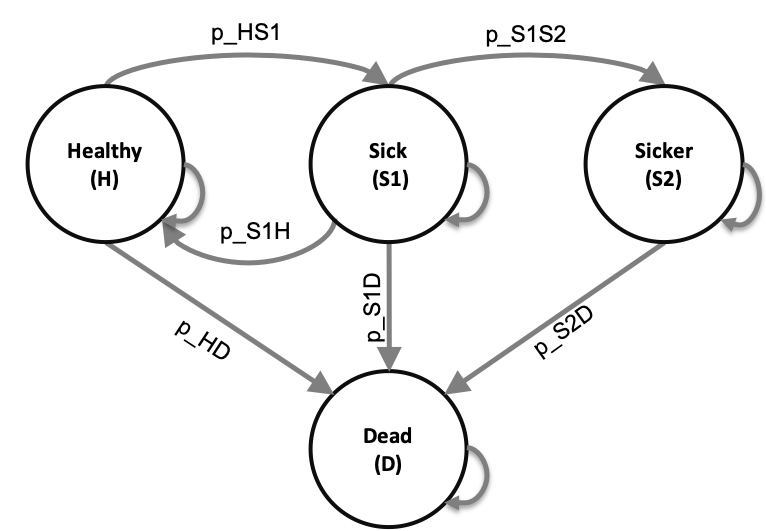
\includegraphics[width=1\linewidth]{C:/Users/Alan Yang/Desktop/GitHub local/Course-Modularization/static/Course_Modularization/Markov models/Markov Sick-Sicker/figures/sick_sicker_diagram} 

}

\caption{Schematic representation of the Sick-Sicker model}\label{fig:unnamed-chunk-1}
\end{figure}

\begin{figure}

{\centering 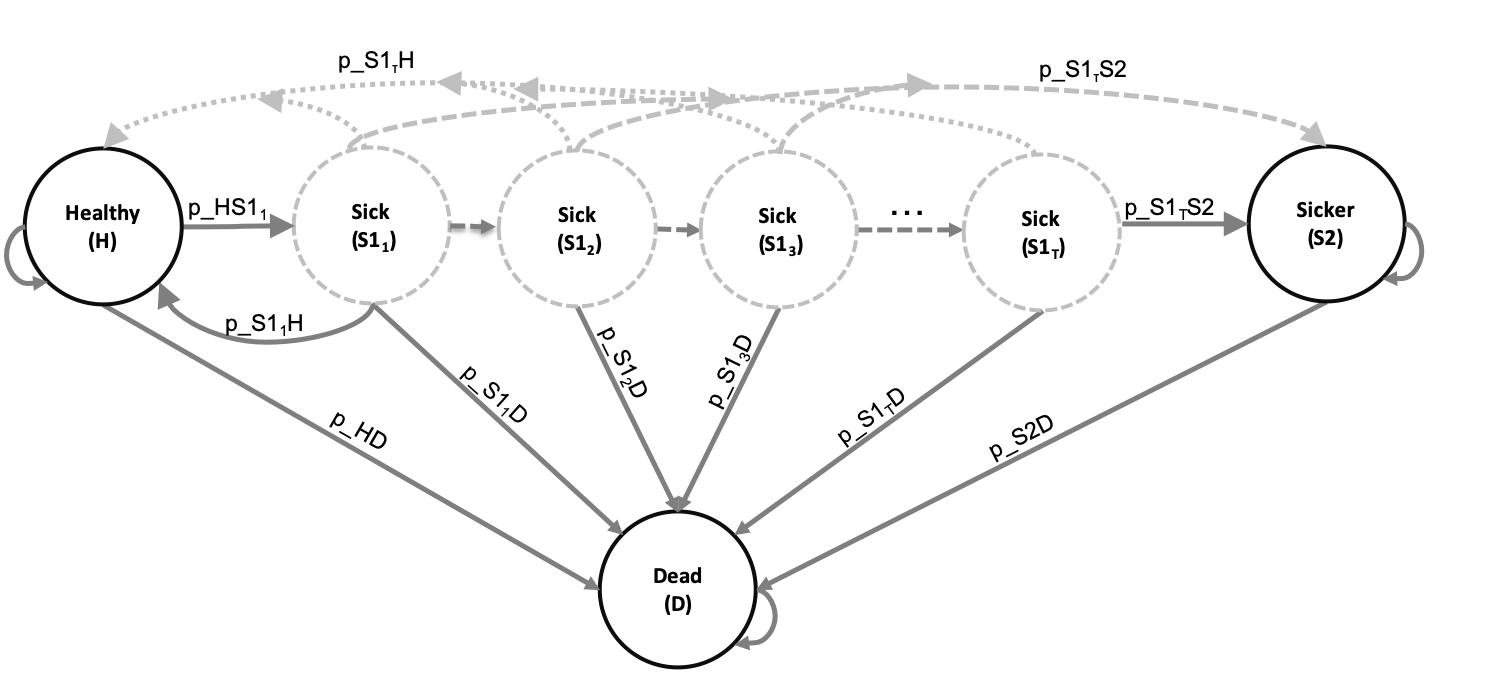
\includegraphics[width=1\linewidth]{C:/Users/Alan Yang/Desktop/GitHub local/Course-Modularization/static/Course_Modularization/Markov models/Markov Sick-Sicker/figures/sick_sicker_tunnels_diagram} 

}

\caption{Schematic representation of the Sick-Sicker model with tunnels states for S1}\label{fig:unnamed-chunk-2}
\end{figure}

\hypertarget{tasks}{%
\subsection{Tasks}\label{tasks}}

\begin{enumerate}
\def\labelenumi{\arabic{enumi}.}
\item
  Starting from the age-dependent Markov model in the R function
  ``Markov\_Sick-Sicker\_time.R'', expand the 3D transition probability
  array to account for tunnels.
\item
  Create the parameter \texttt{p\_S1S2} as a Weibull function as
  follows:
\end{enumerate}

\begin{itemize}
\tightlist
\item
  \texttt{p\_S1S2\ \textless{}-\ l*g*(1:tunnel\_size)\^{}\{g-1\}}, where
\item
  \texttt{l\ \textless{}-\ 0.08} (scale)
\item
  \texttt{g\ \textless{}-\ 1.1} (shape)
\end{itemize}

\begin{enumerate}
\def\labelenumi{\arabic{enumi}.}
\setcounter{enumi}{2}
\item
  Fill in the 3D transition probability array accounting for the tunnel
  states for S1
\item
  Plot the survival curve for the cohort under no treatment. Extra
  challenge: plot the survival curves for all three Markov model
  versions (time-homogenous, age-dependent, and history-dependent) in
  one graph so you can compare.
\end{enumerate}

\begin{longtable}[]{@{}llc@{}}
\toprule
\textbf{Parameter} & \textbf{R name} & \textbf{Value}\tabularnewline
\midrule
\endhead
Time horizon & \texttt{n\_t} & 30 years\tabularnewline
Cycle length & & 1 year\tabularnewline
Names of health states & \texttt{v\_n} & H, S1, S2, D\tabularnewline
Annual discount rate (costs/QALYs) & \texttt{d\_r} & 3\%\tabularnewline
Annual transition probabilities & &\tabularnewline
- Disease onset (H to S1) & \texttt{p\_HS1} & 0.15\tabularnewline
- Recovery (S1 to H) & \texttt{p\_S1H} & 0.5\tabularnewline
- Disease progression (S1 to S2) & \texttt{p\_S1S2} & Weibull
function\tabularnewline
Annual mortality & &\tabularnewline
- All-cause mortality (H to D) & \texttt{p\_HD} &
\texttt{1\ -\ exp(-v\_r\_HD)}\tabularnewline
- Hazard ratio of death in S1 vs H & \texttt{hr\_S1} & 3\tabularnewline
- Hazard ratio of death in S2 vs H & \texttt{hr\_S2} & 10\tabularnewline
Annual costs & &\tabularnewline
- Healthy individuals & \texttt{c\_H} & \$2,000\tabularnewline
- Sick individuals in S1 & \texttt{c\_S1} & \$4,000\tabularnewline
- Sick individuals in S2 & \texttt{c\_S2} & \$15,000\tabularnewline
- Dead individuals & \texttt{c\_D} & \$0\tabularnewline
- Additional costs of sick individuals treated in S1 or S2 &
\texttt{c\_trt} & \$12,000\tabularnewline
Utility weights & &\tabularnewline
- Healthy individuals & \texttt{u\_H} & 1.00\tabularnewline
- Sick individuals in S1 & \texttt{u\_S1} & 0.75\tabularnewline
- Sick individuals in S2 & \texttt{u\_S2} & 0.50\tabularnewline
- Dead individuals & \texttt{u\_D} & 0.00\tabularnewline
Intervention effect & &\tabularnewline
- Utility for treated individuals in S1 & \texttt{u\_trt} &
0.95\tabularnewline
\bottomrule
\end{longtable}

*Note: To calculate the probability of dying from S1 and S2, use the
hazard ratios provided. To do so, first convert the probability of dying
from healthy, \texttt{p\_HD}, to a rate; then multiply this rate by the
appropriate hazard ratio; finally, convert this rate back to a
probability. Recall that you can convert between rates and probabilities
using the following formulas: \(r = -log(1-p)\) and \(p = 1-e^{(-rt)}\)

\hypertarget{exercise-ii-probabilistic-sensitivity-analysis-of-the-sick-sicker-markov-model}{%
\section{Exercise II: Probabilistic sensitivity analysis of the
Sick-Sicker Markov
model}\label{exercise-ii-probabilistic-sensitivity-analysis-of-the-sick-sicker-markov-model}}

This exercise continues based on the age-and-history-dependent
deterministic Markov model of the Sick-Sicker model from Exercise I. In
this exercise, you will do a probabilistic sensitivity analysis (PSA)
with 1000 simulations \texttt{(n\_sim)}. The Table describes the
distributions for the variables you used in the previous exercise.

\textbf{Table II: Input parameters for probabilistic analysis}

\begin{longtable}[]{@{}lrr@{}}
\toprule
\begin{minipage}[b]{0.32\columnwidth}\raggedright
\textbf{Parameter}\strut
\end{minipage} & \begin{minipage}[b]{0.17\columnwidth}\raggedleft
\textbf{Distribution}\strut
\end{minipage} & \begin{minipage}[b]{0.42\columnwidth}\raggedleft
\textbf{Distribution values}\strut
\end{minipage}\tabularnewline
\midrule
\endhead
\begin{minipage}[t]{0.32\columnwidth}\raggedright
Number of simulation\strut
\end{minipage} & \begin{minipage}[t]{0.17\columnwidth}\raggedleft
\texttt{n\_sim}\strut
\end{minipage} & \begin{minipage}[t]{0.42\columnwidth}\raggedleft
1000\strut
\end{minipage}\tabularnewline
\begin{minipage}[t]{0.32\columnwidth}\raggedright
Annual transition probabilities\strut
\end{minipage} & \begin{minipage}[t]{0.17\columnwidth}\raggedleft
\strut
\end{minipage} & \begin{minipage}[t]{0.42\columnwidth}\raggedleft
\strut
\end{minipage}\tabularnewline
\begin{minipage}[t]{0.32\columnwidth}\raggedright
- Disease onset (H to S1)\strut
\end{minipage} & \begin{minipage}[t]{0.17\columnwidth}\raggedleft
Beta\strut
\end{minipage} & \begin{minipage}[t]{0.42\columnwidth}\raggedleft
\(\alpha=30, \ \beta=170\)\strut
\end{minipage}\tabularnewline
\begin{minipage}[t]{0.32\columnwidth}\raggedright
- Recovery (S1 to H)\strut
\end{minipage} & \begin{minipage}[t]{0.17\columnwidth}\raggedleft
Beta\strut
\end{minipage} & \begin{minipage}[t]{0.42\columnwidth}\raggedleft
\(\alpha=60, \ \beta=60\)\strut
\end{minipage}\tabularnewline
\begin{minipage}[t]{0.32\columnwidth}\raggedright
- Disease progression (S1 to S2) in the time-homogeneous model\strut
\end{minipage} & \begin{minipage}[t]{0.17\columnwidth}\raggedleft
Beta\strut
\end{minipage} & \begin{minipage}[t]{0.42\columnwidth}\raggedleft
\(\alpha=84, \ \beta=716\)\strut
\end{minipage}\tabularnewline
\begin{minipage}[t]{0.32\columnwidth}\raggedright
Annual mortality\strut
\end{minipage} & \begin{minipage}[t]{0.17\columnwidth}\raggedleft
\strut
\end{minipage} & \begin{minipage}[t]{0.42\columnwidth}\raggedleft
\strut
\end{minipage}\tabularnewline
\begin{minipage}[t]{0.32\columnwidth}\raggedright
- All-cause mortality (H to D)\strut
\end{minipage} & \begin{minipage}[t]{0.17\columnwidth}\raggedleft
Beta\strut
\end{minipage} & \begin{minipage}[t]{0.42\columnwidth}\raggedleft
\(\alpha=10, \ \beta=1990\)\strut
\end{minipage}\tabularnewline
\begin{minipage}[t]{0.32\columnwidth}\raggedright
- Hazard ratio of death in S1 vs H\strut
\end{minipage} & \begin{minipage}[t]{0.17\columnwidth}\raggedleft
Lognormal\strut
\end{minipage} & \begin{minipage}[t]{0.42\columnwidth}\raggedleft
\(\mu = log(3), \ \sigma = 0.01\)\strut
\end{minipage}\tabularnewline
\begin{minipage}[t]{0.32\columnwidth}\raggedright
- Hazard ratio of death in S2 vs H\strut
\end{minipage} & \begin{minipage}[t]{0.17\columnwidth}\raggedleft
Lognormal\strut
\end{minipage} & \begin{minipage}[t]{0.42\columnwidth}\raggedleft
\(\mu = log(10), \ \sigma = 0.02\)\strut
\end{minipage}\tabularnewline
\begin{minipage}[t]{0.32\columnwidth}\raggedright
Annual costs\strut
\end{minipage} & \begin{minipage}[t]{0.17\columnwidth}\raggedleft
\strut
\end{minipage} & \begin{minipage}[t]{0.42\columnwidth}\raggedleft
\strut
\end{minipage}\tabularnewline
\begin{minipage}[t]{0.32\columnwidth}\raggedright
- Healthy individuals\strut
\end{minipage} & \begin{minipage}[t]{0.17\columnwidth}\raggedleft
Gamma\strut
\end{minipage} & \begin{minipage}[t]{0.42\columnwidth}\raggedleft
shape = 100.0, scale = 20.0\strut
\end{minipage}\tabularnewline
\begin{minipage}[t]{0.32\columnwidth}\raggedright
- Sick individuals in S1\strut
\end{minipage} & \begin{minipage}[t]{0.17\columnwidth}\raggedleft
Gamma\strut
\end{minipage} & \begin{minipage}[t]{0.42\columnwidth}\raggedleft
shape = 177.8, scale = 22.5\strut
\end{minipage}\tabularnewline
\begin{minipage}[t]{0.32\columnwidth}\raggedright
- Sick individuals in S2\strut
\end{minipage} & \begin{minipage}[t]{0.17\columnwidth}\raggedleft
Gamma\strut
\end{minipage} & \begin{minipage}[t]{0.42\columnwidth}\raggedleft
shape = 225.0, scale = 66.7\strut
\end{minipage}\tabularnewline
\begin{minipage}[t]{0.32\columnwidth}\raggedright
- Additional costs of sick individuals treated in S1 or S2\strut
\end{minipage} & \begin{minipage}[t]{0.17\columnwidth}\raggedleft
Gamma\strut
\end{minipage} & \begin{minipage}[t]{0.42\columnwidth}\raggedleft
shape = 73.5, scale = 163.3\strut
\end{minipage}\tabularnewline
\begin{minipage}[t]{0.32\columnwidth}\raggedright
Utility weights\strut
\end{minipage} & \begin{minipage}[t]{0.17\columnwidth}\raggedleft
\strut
\end{minipage} & \begin{minipage}[t]{0.42\columnwidth}\raggedleft
\strut
\end{minipage}\tabularnewline
\begin{minipage}[t]{0.32\columnwidth}\raggedright
- Healthy individuals\strut
\end{minipage} & \begin{minipage}[t]{0.17\columnwidth}\raggedleft
Tr. Normal\strut
\end{minipage} & \begin{minipage}[t]{0.42\columnwidth}\raggedleft
\(\mu = 1.00, \ \sigma = 0.01, \ b = 1\)\strut
\end{minipage}\tabularnewline
\begin{minipage}[t]{0.32\columnwidth}\raggedright
- Sick individuals in S1\strut
\end{minipage} & \begin{minipage}[t]{0.17\columnwidth}\raggedleft
Tr. Normal\strut
\end{minipage} & \begin{minipage}[t]{0.42\columnwidth}\raggedleft
\(\mu = 0.75, \ \sigma = 0.02, \ b = 1\)\strut
\end{minipage}\tabularnewline
\begin{minipage}[t]{0.32\columnwidth}\raggedright
- Sick individuals in S2\strut
\end{minipage} & \begin{minipage}[t]{0.17\columnwidth}\raggedleft
Tr. Normal\strut
\end{minipage} & \begin{minipage}[t]{0.42\columnwidth}\raggedleft
\(\mu = 0.50, \ \sigma = 0.03, \ b = 1\)\strut
\end{minipage}\tabularnewline
\begin{minipage}[t]{0.32\columnwidth}\raggedright
Intervention effect\strut
\end{minipage} & \begin{minipage}[t]{0.17\columnwidth}\raggedleft
\strut
\end{minipage} & \begin{minipage}[t]{0.42\columnwidth}\raggedleft
\strut
\end{minipage}\tabularnewline
\begin{minipage}[t]{0.32\columnwidth}\raggedright
- Utility for treated individuals in S1\strut
\end{minipage} & \begin{minipage}[t]{0.17\columnwidth}\raggedleft
Tr. Normal\strut
\end{minipage} & \begin{minipage}[t]{0.42\columnwidth}\raggedleft
\(\mu = 0.95, \ \sigma = 0.02, \ b = 1\)\strut
\end{minipage}\tabularnewline
\bottomrule
\end{longtable}

\hypertarget{tasks-1}{%
\subsection{Tasks}\label{tasks-1}}

\begin{enumerate}
\def\labelenumi{\arabic{enumi}.}
\setcounter{enumi}{4}
\item
  Create the \texttt{calculate\_ce\_out} \texttt{R} function of the
  Sick-Sicker Markov model in the file
  ``Functions\_markov\_sick-sicker\_tunnels.R''.
\item
  Create a function called \texttt{gen\_psa} to sample values for the
  uncertain parameters using the appropriate distributions. Hint:
  package \texttt{truncnorm} deals with truncated normal distributions.
\item
  Open the file ``markov\_sick-sicker\_tunnels\_SA\_template.R'' and
  conduct a probabilistic Cost-Effectiveness analysis of treatment vs
  no-treatment.
\item
  Create histograms of model inputs.
\item
  Create a cost-effectiveness plane to present discounted costs and
  QALYs.
\item
  Create the cost-effectiveness acceptability curves (CEAC) and frontier
  (CEAF) for the treatment comparison assuming WTP thresholds of \(\$0\)
  to \(\$200,000\).
\item
  Create the expected loss curves (ELCs) plot
\item
  Create an expected value of perfect information (EVPI) plot.
\end{enumerate}

\end{document}
